\apendice{Especificación de Requisitos}

Los requisitos funcionales describen el comportamiento que se desea que el programa tenga, es decir, todas las tareas, servicios o funciones que debe realizar el programa.\cite{malan_functional_2001}

Por otra parte los requisitos no funcionales son aquellos que no definen lo que el software hará sino que se centran en cómo lo hará, por poner unos ejemplos pueden ser requisitos de rendimiento, limitaciones de diseño o características de calidad.\cite{chung2000non} 

\subsection{Catálogo de requisitos}

\subsubsection{Requisitos funcionales}

\begin{itemize}
  \item \textbf{RF-1 Interacción con el modelo:} la interacción con el modelo debe poder realizarse mediante la introducción de prompts al mismo.
  
  \item \textbf{RF-2 Procesamiento del lenguaje natural:} toda interacción con el modelo debe poder realizarse mediante lenguaje natural sin necesidad de código o comandos de ningún tipo, a su vez, las respuestas proporcionadas por el programa deberán estar presentadas en lenguaje natural.
  
  \item \textbf{RF-3 Recuperación de embeddings más significativos:} el programa deberá vectorizar el prompt proporcionado por el usuario, compararlo con los abstract vectorizados en la base de datos y devolver los más significativos, es decir, los abstracts vectorizados cuya distancia al prompt embedido sea menor.
  
  \item \textbf{RF-4 Devolución de respuesta al usuario:} el programa deberá, con el prompt y los abstracts de mayor relevancia, llamar al modelo y generar una respuesta enriquecida la cual será presentada al usuario.
  
  \item \textbf{RF-5 Referencia a la fuente mediante URL en la respuesta:} todos los abstracts recuperados por el modelo deberán ir acompañados con el hipervínculo que redirija al texto completo del artículo mencionado, con ello el usuario puede consultar el texto completo en caso de que quiera profundizar la información con fuentes contrastadas.
  
  \item \textbf{RF-6 Informe de error:} en el caso de que haya algún error en la ejecución del programa o si el usuario introduce un prompt inválido se debe informar al usuario arrojándole el mensaje de error pertinente.
  
  \item \textbf{RF-7 Borrado de conversaciones:} el usuario debe ser capaz de eliminar la última interacción con el programa.
  
  \item \textbf{RF-8 Repetición del prompt:} el usuario debe ser capaz de repetir el prompt previamente introducido de manera cómoda para poder comparar entre diferentes salidas.
  
  \item \textbf{RF-9 Modificación de base de datos vectorizada:} el administrador del programa debe ser capaz de modificar en su totalidad la base de datos vectorizada mediante la cual se realiza el proceso de RAG.

  \item \textbf{RF-10 Afinación de hiperparámetros:} el administrador debe poder modificar el comportamiento del modelo cambiando sus hiperparámetros.

  \item \textbf{RF-11 Inicio de interfaz gráfica:} la interfaz gráfica debe mostrarse tras la ejecución del programa.

  \item \textbf{RF-12 Despliegue en línea:} tras la ejecución del programa, este debe generar un enlace para ser consultado en línea así como compartido entre distintos usuarios.
  
\end{itemize}

\subsubsection{Requisitos no funcionales}

\begin{itemize}
  \item \textbf{RNF-1 Usabilidad:} todo el programa debe contar con funcionalidades lo suficientemente intuitivas como para que un profesional en el ámbito de la salud lo pueda usar sin ningún conocimiento previo en el campo de la computación.
  
  \item \textbf{RNF-2 Mantenibilidad:} el mantenimiento del proyecto debe de estar al alcance de cualquier administrador cualificado encargado de mantener el programa actualizado. También se deben poder realizar mejoras siguiendo el manual del programador incluido en este mismo documento.
  
  \item \textbf{RNF-3 Portabilidad:} el programa debe poder ejecutarse en distintos dispositivos.
  
  \item \textbf{RNF-4 Simultaneidad:} el programa debe poder procesar peticiones provenientes de distintos usuarios.
  
  \item \textbf{RNF-5 Fidelidad:} los artículos presentes en la aplicación deben de provenir de fuentes fiables y contrastadas, al tratarse información sanitaria no se debe dejar al azar las fuentes de información.
  
  \item \textbf{RNF-6 Documentación:} la aplicación debe tener manuales de soporte que faciliten su comprensión y uso.
  
  \item \textbf{RNF-7 Adecuación:} la respuesta proporcionada por el modelo debe estar en sincronía con el prompt proporcionado por el usuario, respondiendo a las preguntas que este propone y realizando las tareas demandadas siempre y cuando estén dentro de las facilidades que el modelo puede proporcionar.

  \item \textbf{RNF-8 Adaptabilidad:} el modelo debe responder correctamente ante modificaciones en la base de datos vectorizada.

  \item \textbf{RNF-9 Decencia:} las respuestas proporcionadas por el modelo deben obedecer a las normas de conducta básicas sin caer en insultos, lenguaje malsonante o desprecio a minorías aunque esto se encuentre en el prompt proporcionado por el usuario.
  
\end{itemize}

\section{Diagrama de casos de uso}

\begin{figure}[h!]
    \centering
    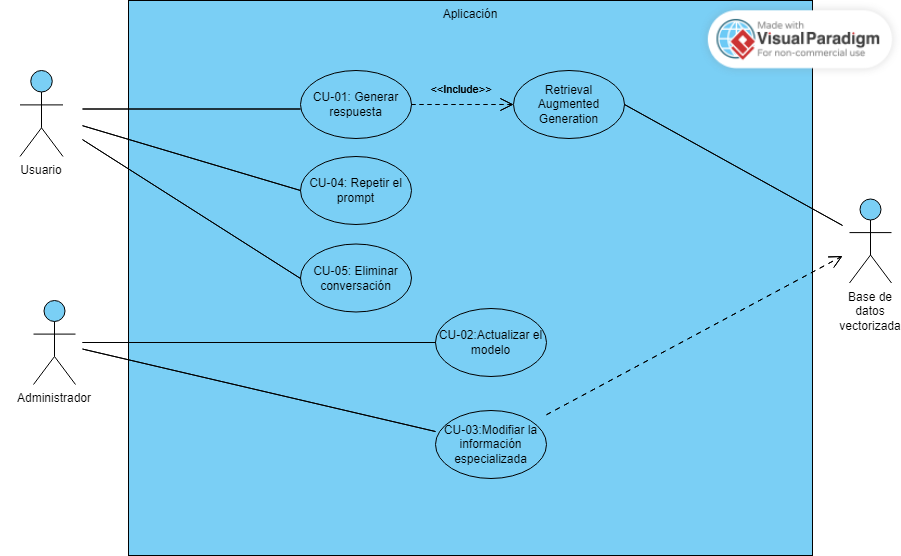
\includegraphics[width=1\textwidth]{img/usecase.png}
    \caption{Diagrama de casos de uso}
    \label{fig:usecase}
\end{figure}

En la figura \ref{fig:usecase} se puede ver un diagrama de casos de uso con tres actores principales, el usuario que es cualquier persona que utilice el programa para generar respuestas a sus cuestiones, el administrador que será el encargado del correcto funcionamiento del proyecto, gestionando los parámetros del modelo así cómo la información que dispone para el enriquecimiento y la base de datos vectorizada donde se almacenan los embeddings de la información con la que queramos enriquecer los prompts con el RAG.

\section{Explicación casos de uso.}

Se puede describir mediante el uso de tablas o mediante lenguaje natural.    

Una muestra de cómo podría ser una tabla de casos de uso:

% Caso de Uso 1 -> Consultar Experimentos.
\begin{table}[p]
	\centering
	\begin{tabularx}{\linewidth}{ p{0.21\columnwidth} p{0.71\columnwidth} }
		\toprule
		\textbf{CU-1}    & \textbf{Generar Respuesta}\\
		\toprule
		\textbf{Versión}              & 1.0    \\
		\textbf{Autor}                & Daniel de Lara Pérez \\
		\textbf{Requisitos asociados} & RF-1, RF-2, RF-3, RF-4, RF-5, RF-6 \\
		\textbf{Descripción}          & El usuario introduce, empleando lenguaje natural, una pregunta o solicitud al programa, esta pregunta se enriquecerá y un modelo generará una respuesta que se devuelve al usuario por pantalla \\
		\textbf{Precondición}         & El proyecto está iniciado \\
		\textbf{Acciones}             &
		\begin{enumerate}
			\def\labelenumi{\arabic{enumi}.}
			\tightlist
			\item El programa recibe la solicitud introducida por el usuario.
			\item Se vectoriza la solicitud para tener una representación matemática de la información.
   		\item El vector se compara, calculando su distancia, con los presentes en la base de datos vectorizada.
     	\item Se devuelve, junto con la solicitud inicial, la información cuya distancia al embedding de la solicitud sea más pequeña.
      	\item La solicitud inicial junto con el prompt son pasados al modelo para enriquecerlo y generar una respuesta especializada.
       	\item Se devuelve la respuesta al usuario.
        	\item El programa queda a la espera de una nueva solicitud.
         
		\end{enumerate}\\
		\textbf{Postcondición}        & La respuesta generada se devuelve al usuario. \\
		\textbf{Excepciones}          & Si el programa recibe una solicitud que no es capaz de procesar como caracteres especiales o lenguaje sin sentido se le informará al usuario \\
		\textbf{Importancia}          & Alta\\
		\bottomrule
	\end{tabularx}
	\caption{CU-1 Generar Respuesta.}
\end{table}

\begin{table}[p]
	\centering
	\begin{tabularx}{\linewidth}{ p{0.21\columnwidth} p{0.71\columnwidth} }
		\toprule
		\textbf{CU-2}    & \textbf{Actualizar el modelo}\\
		\toprule
		\textbf{Versión}              & 1.0    \\
		\textbf{Autor}                & Daniel de Lara Pérez \\
		\textbf{Requisitos asociados} & RF-10 \\
		\textbf{Descripción}          & El administrador modifica el código fuente afinando los valores que se le pasan al modelo como hiperparámetros \\
		\textbf{Precondición}         & El administrador tiene acceso al código fuente \\
		\textbf{Acciones}             &
		\begin{enumerate}
			\def\labelenumi{\arabic{enumi}.}
			\tightlist
			\item El administrador modifica los hiperparámetros por los que considere necesarios.
            \item Se vuelve a ejecutar el código fuente.
         
		\end{enumerate}\\
		\textbf{Postcondición}        & Futuras iteraciones del modelo generan respuestas con los nuevos hiperparámetros. \\
		\textbf{Excepciones}          &  \\
		\textbf{Importancia}          & Alta\\
		\bottomrule
	\end{tabularx}
	\caption{CU-2 Actualizar el modelo.}
\end{table}

\begin{table}[p]
	\centering
	\begin{tabularx}{\linewidth}{ p{0.21\columnwidth} p{0.71\columnwidth} }
		\toprule
		\textbf{CU-3}    & \textbf{Modificar la información especializada}\\
		\toprule
		\textbf{Versión}              & 1.0    \\
		\textbf{Autor}                & Daniel de Lara Pérez \\
		\textbf{Requisitos asociados} & RF-10 \\
		\textbf{Descripción}          & El administrador modifica la información contenida en la base de datos vectorizada, eliminando posibles datos erróneos, añadiendo nueva información o modificando el tema de la especialización. \\
		\textbf{Precondición}         & El administrador tiene acceso al archivo dónde se guarda la información \\
		\textbf{Acciones}             &
		\begin{enumerate}
			\def\labelenumi{\arabic{enumi}.}
			\tightlist
			\item El administrador modifica el archivo añadiendo o eliminando según considere para la tarea que se quiera realizar.
            \item Se vuelve a cargar el archivo con la información (Si el formato en el que se encuentra presentado cambia es posible que haya que modificar también el cargador)
            \item Se tokeniza la información si no se encuentra previamente en tokens establecidos.
            \item Se vuelve a ejecutar el código fuente.
         
		\end{enumerate}\\
		\textbf{Postcondición}        & Futuras iteraciones del modelo generan respuestas especialzadas con la nueva información. \\
		\textbf{Excepciones}          &  \\
		\textbf{Importancia}          & Alta\\
		\bottomrule
	\end{tabularx}
	\caption{CU-3 Modificar la información especializada.}
\end{table}

\begin{table}[p]
	\centering
	\begin{tabularx}{\linewidth}{ p{0.21\columnwidth} p{0.71\columnwidth} }
		\toprule
		\textbf{CU-4}    & \textbf{Repetir el prompt}\\
		\toprule
		\textbf{Versión}              & 1.0    \\
		\textbf{Autor}                & Daniel de Lara Pérez \\
		\textbf{Requisitos asociados} & RF-8 \\
		\textbf{Descripción}          & El usuario repite la misma pregunta para poder contrastar entre dos respuestas diferentes. \\
		\textbf{Precondición}         & El proyecto está iniciado y se ha generado una respuesta \\
		\textbf{Acciones}             &
		\begin{enumerate}
			\def\labelenumi{\arabic{enumi}.}
			\tightlist
			\item El usuario selecciona la opción de repetir el prompt
            \item El programa realiza la misma consulta ya realizada previamente
         
		\end{enumerate}\\
		\textbf{Postcondición}        & El usuario recibe una nueva consulta con el prompt previamente seleccionado. \\
		\textbf{Excepciones}          & No se ha introducido ningún prompt\\
		\textbf{Importancia}          & Media\\
		\bottomrule
	\end{tabularx}
	\caption{CU-4 Repetir el prompt.}
\end{table}

\begin{table}[p]
	\centering
	\begin{tabularx}{\linewidth}{ p{0.21\columnwidth} p{0.71\columnwidth} }
		\toprule
		\textbf{CU-5}    & \textbf{Eliminar conversación}\\
		\toprule
		\textbf{Versión}              & 1.0    \\
		\textbf{Autor}                & Daniel de Lara Pérez \\
		\textbf{Requisitos asociados} & RF-7 \\
		\textbf{Descripción}          & El usuario elimina la última interacción con el modelo o la conversación en su totalidad. \\
		\textbf{Precondición}         & El proyecto está iniciado y se ha generado, al menos, una respuesta \\
		\textbf{Acciones}             &
		\begin{enumerate}
			\def\labelenumi{\arabic{enumi}.}
			\tightlist
			\item El usuario selecciona la opción de eliminar última interacción o toda la conversación
            \item El programa elimina del registro la o las interacciones designadas
         
		\end{enumerate}\\
		\textbf{Postcondición}        & La o las consultas seleccionadas no se muestran por pantalla. \\
		\textbf{Excepciones}          &  No se ha introducido ningún prompt \\
		\textbf{Importancia}          & Baja\\
		\bottomrule
	\end{tabularx}
	\caption{CU-5 Eliminar conversación.}
\end{table}

\section{Prototipos de interfaz o interacción con el proyecto.}

Para este proyecto se ha desarrollado una interfaz de usuario básica que se puede ver en las imágenes \ref{fig:guivacia} y \ref{fig:guirellena}